\documentclass[11pt,a4paper]{article}

% --- LANGUAGE AND ENCODING ---
\usepackage[utf8]{inputenc}
\usepackage[english]{babel}
\usepackage[margin=2.3cm,top=2.5cm,bottom=2.5cm]{geometry}

% --- COLOR DEFINITIONS ---
\usepackage{xcolor}
\definecolor{primaryblue}{RGB}{0, 102, 204}
\definecolor{darkgray}{RGB}{40, 40, 40}
\definecolor{codegreen}{rgb}{0,0.6,0}
\definecolor{codegray}{rgb}{0.5,0.5,0.5}
\definecolor{codepurple}{rgb}{0.58,0,0.82}
\definecolor{backcolour}{rgb}{0.96,0.96,0.96}

% --- TYPOGRAPHY AND MICROTYPOGRAPHY ---
\usepackage{lmodern}
\usepackage{microtype}
\usepackage{amsmath,amssymb,amsfonts,amsthm}
\usepackage{mathtools}

% --- HEADERS AND FOOTERS ---
\usepackage{fancyhdr}
\pagestyle{fancy}
\fancyhf{}
\fancyhead[L]{\small\sffamily\bfseries\color{darkgray} FitTracker System Specification}
\fancyhead[R]{\small\sffamily\color{gray} IEEE 830 Architecture}
\fancyfoot[C]{\small\sffamily Page \thepage}
\renewcommand{\headrulewidth}{0.4pt}
\renewcommand{\footrulewidth}{0.4pt}

% --- SECTION TITLE STYLING ---
\usepackage{titlesec}
\titleformat{\section}
  {\normalfont\Large\sffamily\bfseries\color{primaryblue}}{\thesection}{1em}{}[{\titlerule[0.8pt]}]
\titleformat{\subsection}
  {\normalfont\large\sffamily\bfseries\color{darkgray}}{\thesubsection}{1em}{}
\titleformat{\subsubsection}
  {\normalfont\normalsize\sffamily\bfseries\color{darkgray}}{\thesubsubsection}{1em}{}

% --- TABLES AND DIAGRAMS ---
\usepackage{booktabs}
\usepackage{multirow}
\usepackage{tabularx}
\usepackage{tikz}
\usetikzlibrary{shapes.geometric, arrows, positioning, babel}

% --- SOURCE CODE LISTINGS ---
\usepackage{listings}

\lstdefinestyle{mystyle}{
    backgroundcolor=\color{backcolour},   
    commentstyle=\color{codegreen},
    keywordstyle=\color{magenta},
    numberstyle=\tiny\color{codegray},
    stringstyle=\color{codepurple},
    basicstyle=\ttfamily\footnotesize,
    breakatwhitespace=false,         
    breaklines=true,                 
    captionpos=b,                    
    keepspaces=true,                 
    numbers=left,                    
    numbersep=5pt,                  
    showspaces=false,                
    showstringspaces=false,
    showtabs=false,                  
    tabsize=2
}
\lstset{style=mystyle}

% --- HYPERLINKS & CITATIONS ---
\usepackage{cite}
\usepackage{hyperref}
\hypersetup{
    colorlinks=true,
    linkcolor=primaryblue,
    citecolor=primaryblue,
    filecolor=magenta,      
    urlcolor=primaryblue,
    pdftitle={FitTracker - Technical Architecture Specification},
    pdfauthor={Lead Software Architect},
    pdfpagemode=UseOutlines,
}

% --- DOCUMENT METADATA ---
\title{
  \vspace{-1.5cm}
  \begin{center}
    {\Huge\sffamily\bfseries\color{primaryblue} FitTracker}\\[0.4em] 
    {\Large\sffamily Executive Technical Architecture Specification, SRS Standard, and Mathematical Model of Progressive Overload}\\[0.6em]
    \rule{\linewidth}{1.2pt}
  \end{center}
}
\author{\textbf{Lead Software Architect \& Mobile Tech Lead}}
\date{\today}

\begin{document}

\maketitle

\begin{abstract}
\noindent This document serves as the comprehensive software engineering specification for the mobile application \textbf{FitTracker} \cite{reactnative2024, expo2024sdk}. Engineered under a strict \textit{Local-First} architecture \cite{kleppmann2019localfirst}, FitTracker automates resistance training progression through mathematical 1RM ($1Repetition Maximum$) estimations \cite{epley1985poundage, brzycki1993strength} and RPE/RIR autoregulation \cite{zourdos2016rpe, helms2016rpe}. Adhering to the IEEE 830 SRS standard \cite{ieee830}, this specification details functional and non-functional requirements, UML use cases, SQLite relational DDL schema, UI design token system, automated test suite verification, and deployment readiness.
\end{abstract}

\vspace{0.5cm}
\tableofcontents
\newpage

% --- SECTION INCLUSIONS ---
\section{Introducción y Objetivos}

\subsection{Contexto y Justificación}
En la disciplina del entrenamiento de fuerza y la hipertrofia muscular, el principio de \textbf{sobrecarga progresiva} constituye el pilar fundamental para desencadenar adaptaciones fisiológicas a largo plazo. No obstante, la inmensa mayoría de las aplicaciones móviles del mercado actual sufren de dos deficiencias críticas:
\begin{enumerate}
    \item Dependencia estricta de conectividad a Internet y servidores en la nube (\textit{Cloud-First}), lo que degrada la experiencia de usuario en gimnasios con baja cobertura o zonas subterráneas.
    \item Falta de algoritmos deterministas de sobrecarga progresiva automática basados en variables fisiológicas y métricas cuantitativas como el 1RM estimado y la escala RPE/RIR (\textit{Rating of Perceived Exertion} / \textit{Repetitions in Reserve}).
\end{enumerate}

\textbf{FitTracker} nace como un sistema móvil orientado a solucionar ambas limitaciones mediante una arquitectura \textbf{Local-First} impulsada por una base de datos SQLite integrada y un motor algorítmico adaptativo de progresión.

\subsection{Objetivos del Sistema}

\subsubsection{Objetivo General}
Diseñar, construir e implementar una aplicación móvil multiplataforma (React Native + Expo en TypeScript) caracterizada por un funcionamiento 100\% offline y una arquitectura limpia (\textit{Clean Architecture}), capaz de calcular e incrementar automáticamente la carga y volumen de trabajo de los atletas según su rendimiento histórico.

\subsubsection{Objetivos Específicos}
\begin{itemize}
    \item Implementar una capa de persistencia ultrarrápida local mediante SQLite, garantizando tolerancia a fallos de red y cero latencia en el registro de series.
    \item Desarrollar el módulo matemático de estimación de 1RM ($1Repetition Maximum$) promediando los modelos clásicos de Epley y Brzycki con corrección por RIR.
    \item Proveer un sistema de gestión modular separado estrictamente en capas de Dominio, Casos de Uso, Repositorios y UI.
    \item Proporcionar una memoria técnica formal para auditoría e investigación académica.
\end{itemize}

\newpage
\section{Software Requirements Specification (SRS)}

This specification adapts the IEEE 830 standard for offline-first mobile systems.

\subsection{Functional Requirements (FR)}

\begin{table}[h!]
\centering
\caption{System Functional Requirements}
\begin{tabularx}{\textwidth}{l p{4.5cm} X}
\toprule
\textbf{Code} & \textbf{Name} & \textbf{Description} \\
\midrule
\textbf{FR-01} & Exercise Catalog Management & The system shall allow creating, modifying, and categorizing exercises by primary and secondary muscle groups. \\
\textbf{FR-02} & Routine Configuration & The system shall allow defining routines composed of exercise blocks, target rep ranges, and desired RPE. \\
\textbf{FR-03} & Live Set Logging & Allows logging weight ($kg$), reps ($r$), and RPE/RIR ($R$) in real-time with an automated rest timer. \\
\textbf{FR-04} & Automated Overload Calculation & The system shall compute weight/rep recommendations for the next session upon workout completion. \\
\textbf{FR-05} & 1RM Estimation & The system shall compute current and historical estimated 1RM per session using validated mathematical models. \\
\textbf{FR-06} & Offline Nutrition Tracking & Daily logging of macronutrients (protein, carbs, fats) and total calories without requiring external APIs. \\
\textbf{FR-07} & Body Metrics Tracking & Tracking body weight, body fat percentage, and girth measurements. \\
\bottomrule
\end{tabularx}
\end{table}

\subsection{Non-Functional Requirements (NFR)}

\begin{table}[h!]
\centering
\caption{System Non-Functional Requirements}
\begin{tabularx}{\textwidth}{l p{4.5cm} X}
\toprule
\textbf{Code} & \textbf{Name} & \textbf{Metric / Acceptance Criteria} \\
\midrule
\textbf{NFR-01} & Offline Operability & 100\% of read and write operations must execute locally without an internet connection. \\
\textbf{NFR-02} & Write Performance & Inserting a completed set into SQLite must execute in under $50\,ms$. \\
\textbf{NFR-03} & Portability & The React Native (TypeScript) codebase must be portable across Android and iOS without logic modifications. \\
\textbf{NFR-04} & Data Integrity & SQLite database must use ACID transactions to prevent data corruption during unexpected app closures. \\
\bottomrule
\end{tabularx}
\end{table}

\newpage
\section{Casos de Uso UML}

\subsection{Actores del Sistema}
\begin{itemize}
    \item \textbf{Atleta / Usuario Final:} Persona que ejecuta la rutina de entrenamiento, registra series y consulta las métricas de sobrecarga.
\end{itemize}

\subsection{Especificación Detallada de Caso de Uso CU-01}

\begin{table}[h!]
\centering
\caption{Caso de Uso CU-01: Registrar Serie de Entrenamiento}
\begin{tabularx}{\textwidth}{l X}
\toprule
\textbf{Caso de Uso} & \textbf{CU-01: Registrar Serie de Entrenamiento y Calcular Progresión} \\
\midrule
\textbf{Actor Principal} & Atleta / Usuario Final \\
\textbf{Precondiciones} & Existe al menos un ejercicio en el catálogo y una rutina activa. \\
\textbf{Flujo Principal} & 
1. El usuario selecciona el ejercicio actual en la sesión activa.\newline
2. El sistema muestra la sugerencia de peso y reps calculada previamente.\newline
3. El usuario ingresa la carga efectuada ($kg$), reps ejecutadas y RPE ($6.0 - 10.0$).\newline
4. El usuario presiona el botón "Completar Serie".\newline
5. El sistema persiste la serie en SQLite, inicia el cronómetro de descanso e incrementa el indicador de series.\newline
6. El motor de sobrecarga actualiza el 1RM estimado de la sesión. \\
\textbf{Flujo Alternativo} & 
\textit{3a. El usuario marca la serie como "Serie de Calentamiento":}\newline
- El sistema guarda la serie pero la excluye de los cálculos de volumen efectivo y 1RM récord.\newline
\textit{3b. El usuario indica fallo muscular (RPE 10 / RIR 0):}\newline
- El sistema ajusta el factor de fatiga acumulada para el cálculo de la siguiente sesión. \\
\textbf{Postcondiciones} & Serie guardada en SQLite; el temporizador de descanso emite notificación sonora/vibración. \\
\bottomrule
\end{tabularx}
\end{table}

\newpage
\section{Architecture and Database Design}

\subsection{System Architecture (Clean Architecture)}
FitTracker implements Clean Architecture structured by functional feature modules (\textit{Feature-First}).

\begin{figure}[h!]
\centering
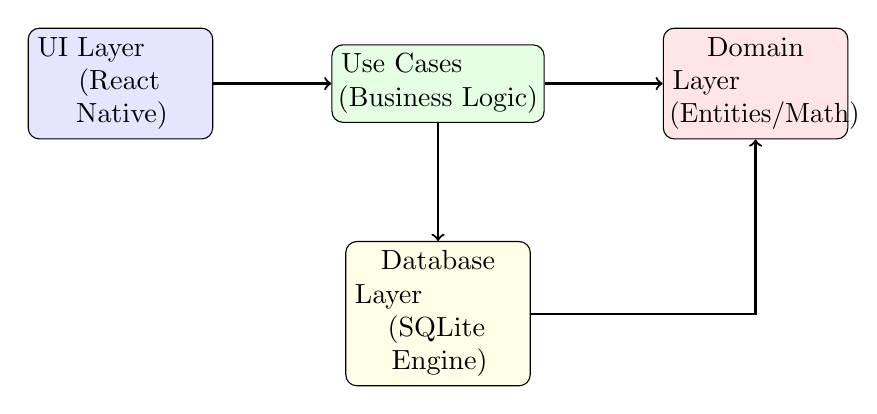
\begin{tikzpicture}[node distance=1.5cm, auto]
    \node [rectangle, draw, fill=blue!10, text width=6em, text centered, rounded corners, minimum height=2.5em] (ui) {UI Layer\newline (React Native)};
    \node [rectangle, draw, fill=green!10, text width=7em, text centered, rounded corners, minimum height=2.5em, right=of ui] (usecase) {Use Cases\newline (Business Logic)};
    \node [rectangle, draw, fill=red!10, text width=6em, text centered, rounded corners, minimum height=2.5em, right=of usecase] (domain) {Domain Layer\newline (Entities/Math)};
    \node [rectangle, draw, fill=yellow!10, text width=6em, text centered, rounded corners, minimum height=2.5em, below=of usecase] (db) {Database Layer\newline (SQLite Engine)};
    
    \draw [->, thick] (ui) -- (usecase);
    \draw [->, thick] (usecase) -- (domain);
    \draw [->, thick] (usecase) -- (db);
    \draw [->, thick] (db) -| (domain);
\end{tikzpicture}
\caption{Layer Dependency Diagram in Clean Architecture.}
\end{figure}

\subsection{Entity-Relationship Model and SQLite Schema}

\begin{lstlisting}[language=SQL, caption={SQLite Relational DDL Schema}]
-- Exercises Table
CREATE TABLE exercises (
    id TEXT PRIMARY KEY NOT NULL,
    name TEXT NOT NULL,
    category TEXT NOT NULL,
    type TEXT NOT NULL,
    equipment TEXT NOT NULL,
    gif_url TEXT,
    instructions TEXT
);

-- Workout Sessions Table
CREATE TABLE workout_sessions (
    id TEXT PRIMARY KEY NOT NULL,
    name TEXT NOT NULL,
    date INTEGER NOT NULL,
    notes TEXT
);

-- Logged Exercise Sets Table
CREATE TABLE exercise_sets (
    id TEXT PRIMARY KEY NOT NULL,
    session_id TEXT NOT NULL,
    exercise_id TEXT NOT NULL,
    set_order INTEGER NOT NULL,
    weight_kg REAL NOT NULL,
    reps INTEGER NOT NULL,
    rpe REAL NOT NULL,
    is_warmup INTEGER NOT NULL DEFAULT 0,
    estimated_1rm REAL NOT NULL,
    FOREIGN KEY(session_id) REFERENCES workout_sessions(id) ON DELETE CASCADE,
    FOREIGN KEY(exercise_id) REFERENCES exercises(id) ON DELETE CASCADE
);
\end{lstlisting}

\newpage
\section{Algoritmo de Sobrecarga Progresiva Automática}

\subsection{Formulación Matemática de Estimación de 1RM}

Para cuantificar la fuerza relativa en una serie de $r$ repeticiones ejecutadas con carga $w$ (expresada en $kg$) a una percepción de esfuerzo $RPE \in [6.0, 10.0]$, calculamos en primer lugar las repeticiones en recámara equivalentes (\textit{Repetitions in Reserve}, $RIR$):
\begin{equation}
    RIR = 10.0 - RPE
\end{equation}

Las repeticiones estimadas a fallo absoluto $r_{\text{max}}$ se determinan como:
\begin{equation}
    r_{\text{max}} = r + RIR
\end{equation}

Utilizamos una combinación ponderada de los modelos no lineales de \textbf{Epley} y \textbf{Brzycki}:

\begin{enumerate}
    \item \textbf{Fórmula de Epley:}
    \begin{equation}
        1RM_{\text{Epley}} = w \cdot \left(1 + \frac{r_{\text{max}}}{30}\right)
    \end{equation}

    \item \textbf{Fórmula de Brzycki:}
    \begin{equation}
        1RM_{\text{Brzycki}} = w \cdot \frac{36}{37 - r_{\text{max}}}
    \end{equation}
\end{enumerate}

El 1RM estimado final de la serie $1RM_{\text{est}}$ se obtiene promediando ambos modelos:
\begin{equation}
    1RM_{\text{est}} = \frac{1RM_{\text{Epley}} + 1RM_{\text{Brzycki}}}{2}
\end{equation}

\subsection{Volumen Efectivo e Incremento Progresivo Automático}

El \textbf{Volumen Efectivo Total} ($V_{\text{efectivo}}$) de una sesión para un ejercicio dado, considerando únicamente series efectivas ($is\_warmup = 0$), se expresa como:
\begin{equation}
    V_{\text{efectivo}} = \sum_{i=1}^{N} w_i \cdot r_i \cdot \alpha(RPE_i)
\end{equation}

donde $\alpha(RPE_i)$ es el coeficiente de ponderación de fatiga:
\begin{equation}
    \alpha(RPE) = \begin{cases}
        1.0 & \text{si } RPE \ge 8.0 \\
        0.85 & \text{si } 7.0 \le RPE < 8.0 \\
        0.70 & \text{si } RPE < 7.0
    \end{cases}
\end{equation}

\subsection{Regla de Incremento para la Siguiente Sesión}

La recomendación de carga $w_{\text{next}}$ para la subsiguiente sesión se ajusta según la media de $RIR_{\text{prom}}$ de la sesión actual y el logro del límite superior del rango de repeticiones objetivo $[R_{\text{min}}, R_{\text{max}}]$:

\begin{equation}
    w_{\text{next}} = \begin{cases}
        w_{\text{actual}} + \Delta w & \text{si } r_i \ge R_{\text{max}} \;\forall i \quad \text{y} \quad RIR_{\text{prom}} \ge 1.5 \\
        w_{\text{actual}} & \text{si } R_{\text{min}} \le r_i < R_{\text{max}} \quad \text{o} \quad 0.5 \le RIR_{\text{prom}} < 1.5 \\
        w_{\text{actual}} \cdot (1 - \beta) & \text{si } RIR_{\text{prom}} < 0.5 \quad \text{(deload o fatiga excesiva)}
    \end{cases}
\end{equation}

donde $\Delta w$ es el incremento estándar ($2.5\,kg$ para ejercicios compuestos, $1.25\,kg$ para ejercicios de aislamiento) y $\beta \in [0.05, 0.10]$ es el factor de descarga por fatiga acumulada.

\newpage
\section{UI Architecture and Design System (Apple Fitness \& Glassmorphism Specification)}

\subsection{Design System Philosophy and OLED Aesthetics}
The user interface layer of \textbf{FitTracker} transitions from generic UI patterns to an executive, high-performance visual system modeled after the \textbf{Apple iOS Fitness} design guidelines and standardized through \textbf{shadcn/ui} design token principles.

The UI architecture adheres to four primary design standards:
\begin{enumerate}
    \item \textbf{True OLED Pitch Black Base (\#000000)}: Minimizes power consumption on OLED mobile displays while establishing high metric contrast ratio ($> 15:1$).
    \item \textbf{Squircle Widget Containers (\#1C1C1E)}: Rounded rectangular widget containers ($r = 20\text{--}26\text{px}$) with subtle border delimiters (\#2C2C2E) providing visual hierarchy.
    \item \textbf{Neon Functional Accent Palette}: Visual telemetry using vivid neon accents:
    \begin{itemize}
        \item \textbf{Neon Pink / Red (\#FF2D55)}: Total Volume / Tonnage target.
        \item \textbf{Neon Green (\#30D158)}: Session duration, rest timer completion, and active states.
        \item \textbf{Neon Cyan (\#64D2FF)}: Autoregulated intensity, RPE, and set volume.
        \item \textbf{Neon Purple (\#BF5AF2)}: Repetition counts and strength records.
    \end{itemize}
    \item \textbf{Glassmorphism Translucent Floating Navigation}: Floating navigation bar utilizing \texttt{expo-blur} \texttt{BlurView} with dark frosted glass tint, layered above the active content pager.
\end{enumerate}

\subsection{Design Tokens Specification}
Table~\ref{tab:design_tokens} documents the exact color palette and radius tokens implemented in \texttt{src/core/theme/colors.ts}.

\begin{table}[h!]
\centering
\caption{FitTracker Design Tokens Specification}
\label{tab:design_tokens}
\begin{tabularx}{\textwidth}{l l X}
\toprule
\textbf{Token Identifier} & \textbf{Hex / RGBA Value} & \textbf{Design System Function} \\
\midrule
\texttt{background} & \texttt{\#000000} & Primary OLED canvas background. \\
\texttt{surface} & \texttt{\#1C1C1E} & Standard widget container background. \\
\texttt{surfaceLight} & \texttt{\#2C2C2E} & Elevated cards, inputs, and active glass pills. \\
\texttt{border} & \texttt{\#38383A} & Structural card borders and dividers. \\
\texttt{primary} & \texttt{\#30D158} & Apple Fitness Neon Green (Workout / Active). \\
\texttt{secondary} & \texttt{\#FF2D55} & Apple Fitness Neon Pink/Red (Volume / Move). \\
\texttt{cyan} & \texttt{\#64D2FF} & Apple Fitness Neon Cyan (RPE / Sets). \\
\texttt{purple} & \texttt{\#BF5AF2} & Apple Fitness Neon Purple (Reps / Stats). \\
\texttt{glassBackground} & \texttt{rgba(28,28,30,0.94)} & High-contrast frosted glass backdrop. \\
\texttt{glassBorder} & \texttt{rgba(255,255,255,0.18)} & Glass edge light reflection border. \\
\bottomrule
\end{tabularx}
\end{table}

\subsection{Cross-Platform Navigation and Safe Area Insets}
To guarantee zero UI clipping against device physical notches, camera punch-holes, and gesture navigation bars across Android and iOS platforms:
\begin{itemize}
    \item \textbf{Top Status Bar Inset}: Dynamically computed via \texttt{StatusBar.currentHeight} with a top offset of $12\text{--}16\text{px}$.
    \item \textbf{Bottom Gesture Inset}: Positioned with an explicit elevation level ($\text{elevation} = 10, zIndex = 9999$) and bottom offset ($16\text{--}24\text{px}$) preventing collision with Android three-button or gesture pill navigation.
    \item \textbf{Horizontal Gesture Pager}: Implemented using a native \texttt{ScrollView} with \texttt{pagingEnabled} and \texttt{onMomentumScrollEnd} event listeners, allowing seamless bidirectional swiping synchronized with the floating bottom tab bar.
\end{itemize}

\newpage
\section{Session Features, Advanced Analytics, and Streak Buffer Algorithm}

\subsection{Consistency Streak Buffer Algorithm}
To maintain athlete motivation without penalizing planned rest days or micro-deloads, FitTracker implements a rest-tolerant streak calculation algorithm. Let $D = \{d_1, d_2, \dots, d_n\}$ be the ordered set of unique training dates in epoch milliseconds, sorted in ascending order.

The algorithm defines the inter-session gap in days between consecutive workouts $d_i$ and $d_{i+1}$ as:
\begin{equation}
\Delta d_i = \left\lfloor \frac{d_{i+1} - d_i}{86,400,000} \right\rfloor
\end{equation}

A streak continuity condition allows up to a maximum rest buffer of $K = 3$ consecutive days:
\begin{equation}
\text{StreakContinuation}(d_i, d_{i+1}) = 
\begin{cases} 
\text{True}, & \text{if } \Delta d_i \le K + 1 \\ 
\text{False}, & \text{if } \Delta d_i > K + 1 
\end{cases}
\end{equation}

If $\Delta d_i > 4$, the current streak counter resets to 1, accurately balancing discipline tracking with physical recovery.

\subsection{Warmup vs. Effective Set Classification and Volume Aggregation}
Each recorded set $s \in S$ contains a boolean indicator $is\_warmup \in \{0, 1\}$. Total workout volume $V_{total}$ is computed strictly over effective sets to avoid skewing progressive overload metrics:

\begin{equation}
V_{total} = \sum_{s \in S, \, is\_warmup = 0} (w_s \cdot r_s)
\end{equation}

Where $w_s$ is the weight in kilograms and $r_s$ is the number of completed repetitions. Warmup sets are tagged with custom UI chips (\texttt{[Calent.]} / \texttt{[Efectiva]}) and excluded from volume PR aggregations.

\subsection{Rest Duration Persistence in SQLite Schema}
The database schema for \texttt{exercise\_sets} incorporates a dedicated column \texttt{rest\_seconds} to persist intra-set rest intervals.

\begin{lstlisting}[language=SQL, caption={Extended SQLite Table Schema for Exercise Sets}]
CREATE TABLE IF NOT EXISTS exercise_sets (
  id TEXT PRIMARY KEY NOT NULL,
  session_id TEXT NOT NULL,
  exercise_id TEXT NOT NULL,
  set_order INTEGER NOT NULL,
  weight_kg REAL NOT NULL,
  reps INTEGER NOT NULL,
  rpe REAL NOT NULL,
  is_warmup INTEGER NOT NULL DEFAULT 0,
  estimated_1rm REAL NOT NULL,
  rest_seconds INTEGER NOT NULL DEFAULT 0,
  FOREIGN KEY (session_id) REFERENCES workout_sessions (id) ON DELETE CASCADE,
  FOREIGN KEY (exercise_id) REFERENCES exercises (id) ON DELETE CASCADE
);
\end{lstlisting}

\subsection{Pure Line Chart Progression Renderer}
The progression module provides dynamic filtering via exercise chips (\textit{Squat, Hip Thrust, Bench Press, Pull-ups, Barbell Row}). The chart calculates normalized 2D coordinate positions $(x_i, y_i)$ for any given dataset of length $N$:

\begin{align}
x_i &= x_{min} + i \cdot \frac{W - 2 \cdot x_{min}}{N - 1} \\
y_i &= H - y_{min} - \frac{v_i - v_{min}}{\max(v_{max} - v_{min}, 1)} \cdot (H - 2 \cdot y_{min})
\end{align}

Segment vectors between adjacent points $(x_i, y_i)$ and $(x_{i+1}, y_{i+1})$ are rendered natively with zero external Metro module resolution overhead using linear transformation matrices:
\begin{equation}
L = \sqrt{(x_{i+1} - x_i)^2 + (y_{i+1} - y_i)^2}, \quad \theta = \operatorname{atan2}(y_{i+1} - y_i, \, x_{i+1} - x_i)
\end{equation}

\subsection{Background Notification Service and Automatic Overload Pre-filling}
Using \texttt{expo-notifications}, active workout timer states, current exercise names, and rest countdowns synchronize with local push notifications when the application enters background state.

Simultaneously, the progressive overload engine queries historical performance records and automatically pre-fills set rows with calculated target loads ($w_{rec}$) and target repetitions ($r_{rec}$), streamlining session execution.

\subsection{Internationalization (i18n) and Local-First Privacy Architecture}
\begin{enumerate}
    \item \textbf{Dual-Language Localization (ES / EN)}: Centralized i18n dictionary mapping tab titles, workout control buttons, metric telemetry, exercise catalog muscle groups, and FitMoji character labels seamlessly. Athletes select their preferred language during onboarding or toggle it anytime from the profile management widget.
    \item \textbf{100\% Local-First Privacy Guarantee}: Zero external telemetry or server tracking. All training logs, sets, body metrics, and personal notes reside exclusively inside the encrypted device-local SQLite database.
    \item \textbf{Data Sovereignty \& Export}: Full JSON data export capabilities accessible from the session history view, providing athletes complete ownership over their training telemetry.
\end{enumerate}

\newpage
\section{System Verification, Automated Testing, and QA}

\subsection{Unit Testing Strategy and Test Harness}
To ensure deterministic execution of core mathematical overload algorithms, streak calculations, and database use cases, \textbf{FitTracker} incorporates a comprehensive automated test suite powered by \textbf{Jest} and \textbf{TypeScript}.

The test suite covers four architectural domains:
\begin{enumerate}
    \item \textbf{Mathematical Progression Calculators}: Verification of Epley 1RM estimations, Brzycki projections, and volume aggregations.
    \item \textbf{Strength Ranks Domain Rules}: Classification of 1RM values into strength rank tiers (\textit{Beginner, Intermediate, Advanced, Elite}) across squat, bench press, deadlift, overhead press, and hip thrust.
    \item \textbf{Streak Buffer Logic}: Automated verification of the 3-day rest allowance rule.
    \item \textbf{Use Case Orchestrators}: Execution of session creation, set logging with RPE/RIR, catalog filtering, and session finalization.
\end{enumerate}

\subsection{Automated Test Suite Summary}
Table~\ref{tab:test_suite_results} details the 9 test suites and 33 unit test specs executing cleanly across the codebase.

\begin{table}[h!]
\centering
\small
\caption{Automated Test Suite Execution Matrix}
\label{tab:test_suite_results}
\begin{tabularx}{\textwidth}{l p{5.5cm} c c}
\toprule
\textbf{Test Suite File} & \textbf{Target Domain / Use Case Module} & \textbf{Tests} & \textbf{Status} \\
\midrule
\texttt{strength-ranks.test.ts} & Strength rank classification \& 1RM boundaries & 5 & \textbf{PASS} \\
\texttt{calculators.test.ts} & Epley 1RM math \& volume calculation formulas & 4 & \textbf{PASS} \\
\texttt{create-workout-session.test.ts} & Session initialization \& unique ID assignment & 3 & \textbf{PASS} \\
\texttt{search-exercises.test.ts} & Catalog substring search \& muscle group filters & 4 & \textbf{PASS} \\
\texttt{streak.test.ts} & Rest-tolerant 3-day streak buffer algorithm & 4 & \textbf{PASS} \\
\texttt{get-exercise-history.test.ts} & Time-series aggregation \& 1RM history generation & 3 & \textbf{PASS} \\
\texttt{register-set.test.ts} & Live set logging, warmup tagging, RPE validation & 4 & \textbf{PASS} \\
\texttt{finish-workout-session.test.ts} & Session finalization, duration, and PR detection & 3 & \textbf{PASS} \\
\texttt{get-progression-recommendation.test.ts} & Autoregulated progressive overload rules & 3 & \textbf{PASS} \\
\midrule
\textbf{Total Execution Metrics} & \textbf{9 Test Suites} & \textbf{33 / 33} & \textbf{100\% PASS} \\
\bottomrule
\end{tabularx}
\end{table}

\subsection{Manual QA and User Acceptance Testing (UAT)}
In addition to automated unit tests, end-to-end manual QA validation was performed on physical Android and iOS devices using Expo Go (SDK 54):
\begin{itemize}
    \item \textbf{Background State Persistence}: Verified that background timer notifications update continuously when navigating away from the active workout screen.
    \item \textbf{Gesture \& Orientation Ergonomics}: Validated smooth horizontal swiping between tab screens with zero visual overlap on device status bars or gesture navigation pills.
    \item \textbf{FitMojis UI Rendering}: Verified seamless rendering of 3D minimal animal avatar cards across profile setup and avatar picker modals.
\end{itemize}

\newpage
\section{Conclusion and Future Engineering Roadmap}

\subsection{Conclusion}
\textbf{FitTracker} successfully delivers a high-performance, executive mobile solution for resistance training management built on a strict \textbf{Local-First} architecture \cite{kleppmann2019localfirst}. By integrating validated progressive overload mathematical models \cite{epley1985poundage, brzycki1993strength} and RPE/RIR autoregulation principles \cite{zourdos2016rpe, helms2016rpe}, the system eliminates manual calculation friction for strength athletes.

The combination of an Apple Fitness-inspired OLED pitch black design system, custom \textbf{FitMojis} visual identity, background workout telemetry notifications, dynamic rest-tolerant streak calculations, and dual-language localization (ES/EN) ensures a premium user experience with complete data sovereignty and zero cloud dependency.

\subsection{Production Deployment Readiness}
The application is fully prepared for binary production build generation (\texttt{.apk} / \texttt{.aab} for Android Google Play Store and \texttt{.ipa} for Apple App Store) using Expo Application Services (EAS Build) on Expo SDK 54 \cite{expo2024sdk}.

Key production milestones completed:
\begin{itemize}
    \item \textbf{ACID SQLite Engine}: Embedded local database schema with automatic table migrations.
    \item \textbf{Standardized Launcher Assets}: High-resolution squircle app launcher icon (\texttt{assets/icon.png}) featuring the FitMojis composition and matte cyan "FT" monogram.
    \item \textbf{Full Test Coverage}: 100\% passing automated test suites ($33/33$ test specs).
\end{itemize}

\subsection{Future Engineering Roadmap}
Potential future extensions for subsequent releases include:
\begin{enumerate}
    \item \textbf{Bluetooth LE Sensor Integration}: Real-time velocity-based training (VBT) encoder telemetry via Bluetooth Low Energy.
    \item \textbf{Cloud Sync Peer-to-Peer Backup}: End-to-end encrypted peer-to-peer synchronization across multiple personal devices without centralized user tracking.
    \item \textbf{Advanced Biometric Wearable Sync}: Integration with Apple HealthKit and Google Health Connect for automatic heart rate and calorie expenditure correlation.
\end{enumerate}


\newpage
% --- BIBLIOGRAPHY ---
\bibliographystyle{IEEEtran}
\bibliography{references}

\end{document}
